\documentclass[11pt]{amsart}

% Standard letter size paper with 1inch margins
\usepackage[letterpaper, margin=1in]{geometry}
\usepackage{booktabs} % For better looking tables
\usepackage{xcolor}
\usepackage{pifont}

% Useful packages 
\usepackage{amsmath, amssymb, amsthm, amsaddr}
\usepackage{enumerate, subcaption, graphicx, hyperref}
\usepackage{algorithm}
\usepackage{algpseudocode}
\usepackage{cite}
\usepackage{bm}

\newcommand{\I}{\mathrm{i}}
\DeclareMathOperator{\E}{e}

\title{AMATH 582: Homework 4}
\author{Hunter Lybbert} % first and last name

\address{Applied Mathematics Department, University of Washington, Seattle, WA 
\\ \texttt{hlybbert@uw.edu}}

\date{\today} % you can also just type the date instead of "\today"

\begin{document}

\maketitle

\begin{abstract}
    In this report we survey fully connected linear neural networks and the most common hyperparameters to consider for tuning.
    Various methods of optimization are evaluated with a variety of learning rates and momentums.
    Dropout and batch normalization are discussed and implemented as well.
    Methods of hyperparameter tuning, comparing models and results are presented.
    The task we are applying this to is the well known 10 class classification problem with the FashionMNIST dataset.
\end{abstract}

\section{Introduction and Overview}\label{sec:Introduction}
In this report we further our understanding of machine learning concepts focusing on deep learning, the study of neural network based model architecture.

Again, our setup is a common supervised learning problem, given a collection of $N$ data points with labels in classification or target values in a regression setting $$\big\{(\bm{x_0}, y_0), (\bm{x_1}, y_1), ..., (\bm{x_{N-1}}, y_{N-1})\big\}.$$
The data is denoted as a matrix $X$ and a vector of target values or class labels $\bm y$.
We then are looking for a function $f$ which takes in the training data and most accurately predicts the target values or class labels, written in optimization form we are looking for the following
$$f_{MLE} = \underset{f}{\rm argmin } \frac 1 {2 \sigma^2}|| f(X) - \bm y ||_2^2$$
where $\sigma^2$ is the variance of the normally distributed error terms $\epsilon \sim \mathcal N (0, \sigma^2)$ defined by $\epsilon_i = y_i - f(x_i)$.
So said another way we are trying to minimize our errors in the classification task.
The specific class of functions $f$ to be considered to solve the problem is a Fully Connected Neural Network (FCN).
We will treat the theoretical background of these methods in the next section.

Before proceeding, we would like to acknowledge the critical use of the following packages in our analysis.
Namely, Matplotlib was used to create all plots and animations \cite{Hunter:2007}.
\textbf{TODO: Add ray tune and pytorch...!}
Additionally, Scikit-learn was the primary source of using the PCA algorithm and other classification methods \cite{scikit-learn}.

%\begin{figure}[h]
%	\centering
%	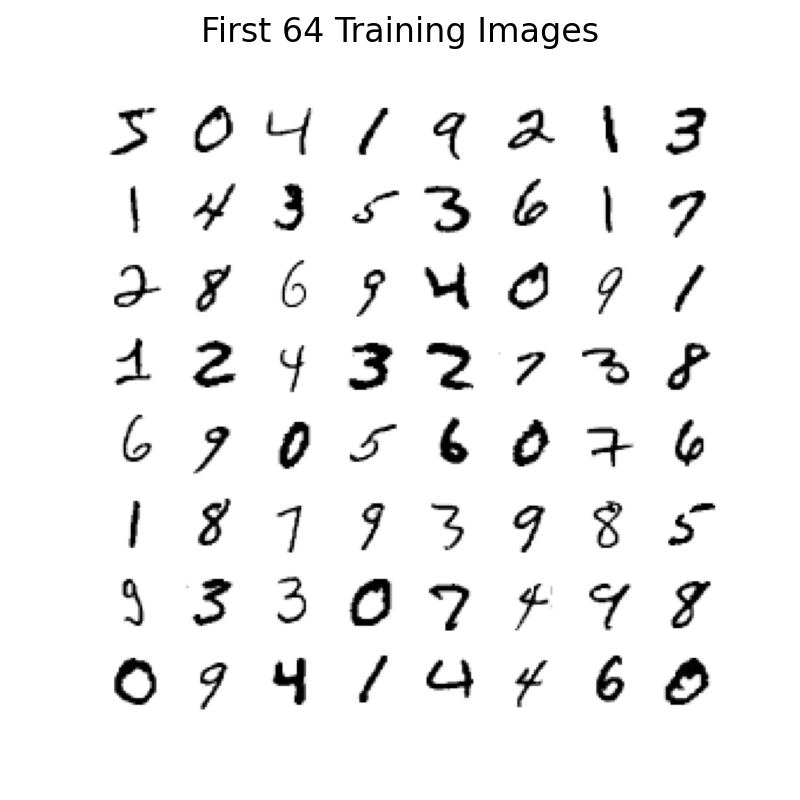
\includegraphics[width=.5\textwidth]{../visualizations/first_64_training_images.png}
% 	\caption{ As an insight to the problem at hand I have visualized the first 64 training images.
%	Not included in this report but available on my GitHub are animated visualizations of all training samples for a given digit. Something interesting that this revealed is that many of the training samples for the digit 2, us the curly circular style in the lower left hand corner of the symbol. This is notable because that makes a starker difference between 2 and 7 than we would expect. This could explain why 2 and 7 are easier to diliminate than we assumed. }\label{fig:f3}
%\end{figure}

\section{Theoretical Background}\label{sec:theory}
\textbf{TODO: General background about the idea of neural networks}

\subsection{Architecture}
\textbf{TODO: Update}

\subsection{Optimizer}
\textbf{TODO: Update}

\subsection{Learning Rate}
\textbf{TODO: Update}

\subsection{Momentum}
\textbf{TODO: Update}

\subsection{Dropout}
\textbf{TODO: Update}

\subsection{Batch Normalization}
\textbf{TODO: Update}

\section{Algorithm Implementation and Development}\label{sec:algorithms}
\textbf{TODO: Update}

%\begin{figure}[h]
%	\centering
%	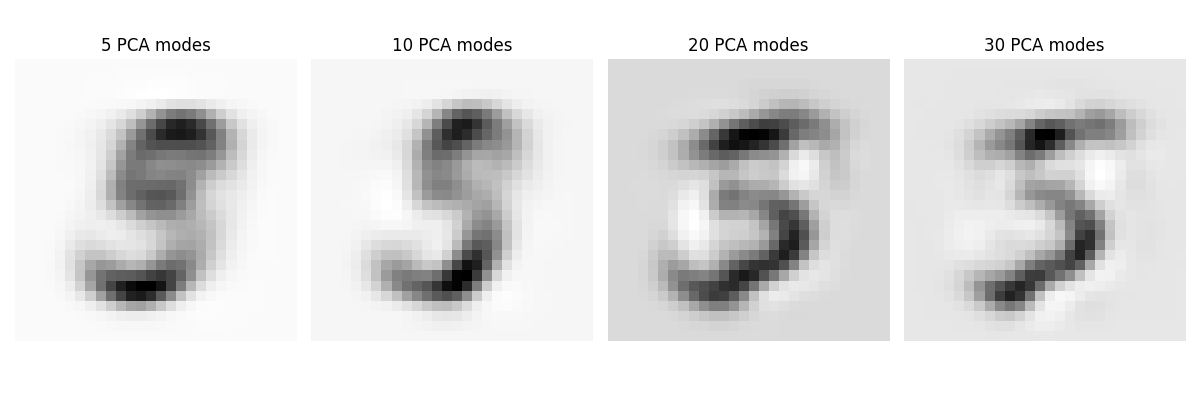
\includegraphics[width=.5\textwidth]{../visualizations/digit_reconstruction.png}
% 	\caption{ An analysis of how much information or energy is retained in our data matrix given a certain number of components are used in the PCA transformation.
%	We have visualized the reconstructed images after they've been projected to k-pc mode space and inversed to the original space.
%	We can see the 59 pc modes really do retain a large amount of information (85\% as calculated using the cumulative energy)}\label{fig:f0}
%\end{figure}


%\begin{figure}[h]
%    \centering
%    \begin{subfigure}{0.4\textwidth}
%        \centering
%        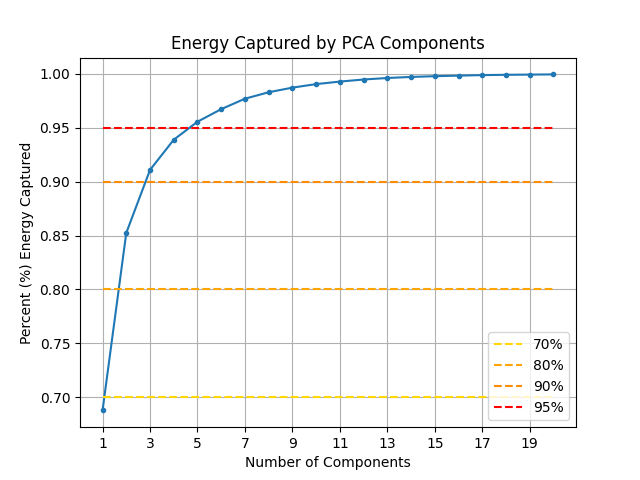
\includegraphics[width=\textwidth]{../visualizations/energy_by_components.png}
%        \label{fig:image1}
%    \end{subfigure}
%    \caption{ This is the percentage of Total Energy which is preserved by projecting our digit images into a given number of pc modes. 
%    We were tasked to calculate the minimum number of pc modes needed to be kept in order to retain 85\% of the total energy or information from the original image.
%    As displayed with the orange star overlayed on the plot, the minimum number of pc components needed are 59.}
%    \label{fig:f1}
%\end{figure}

\section{Computational Results}\label{sec:results}

\textbf{TODO: Update}

%\begin{table}[h]
%    \centering
%    \begin{tabular}{|l|c|c|c|c|} % 'l' for left-aligned, 'c' for center-aligned columns
%        \hline
%        \textbf{Classifier} & \textbf{Digits Used} & \textbf{Train Accuracy} & \textbf{Test Accuracy} & \textbf{CV Score} \\ 
%        \hline
%        Ridge Classifier & 1 and 8 & 0.965  & 0.980 & 0.963 $\pm$ 0.00281 \\
%        \hline
%        Ridge Classifier & 3 and 8 & 0.961  & 0.964 & 0.959 $\pm$ 0.00590 \\
%        \hline
%        Ridge Classifier & 2 and 7 & 0.981  & 0.973 & 0.981 $\pm$ 0.00226 \\  
%        \hline
%    \end{tabular}
%    \caption{The performance of RidgeClassifier on different binary digit classification problems. First evaluated on the task of distinguishing between 1 and 8, followed by 3 and 8, then finally 2 and 7.}
%    \label{tab:tab0}
%\end{table}

%\begin{table}[h]
%    \centering
%    \begin{tabular}{|l|c|c|c|} % 'l' for left-aligned, 'c' for center-aligned columns
%        \hline
%        \textbf{Classifier} & \textbf{Train Accuracy} & \textbf{Test Accuracy} & \textbf{CV Score} \\ 
%        \hline
%        Ridge Classifier & 0.845  & 0.856 & 0.844 $\pm$ 0.00997 \\  
%        \hline
%        K-nearest Neighbors & 0.986 & 0.976 \textcolor{red}{\ding{72}} & 0.975 $\pm$ 0.00109 \\
%        \hline
%        Linear Discriminant Analysis & 0.866 & 0.875 & 0.865 $\pm$ 0.00870 \\  
%        \hline
%        Random Forest Classifier & 0.998 & 0.947 & 0.942 $\pm$ 0.00407 \\  
%        \hline
%        Gradient Boosting Classifier & 0.939 & 0.928 & 0.918 $\pm$ 0.00554 \\  
%        \hline
%    \end{tabular}
%    \caption{The performance of each model on the full digit recognition task, aka multi-class classification of digits.
%    Using the performance on the test set as our selection metric, I would conclude that K-nearest Neighbors performed best on this classification task.}
%    \label{tab:tab1}
%\end{table}


%\begin{figure}[h]
%	\centering
%	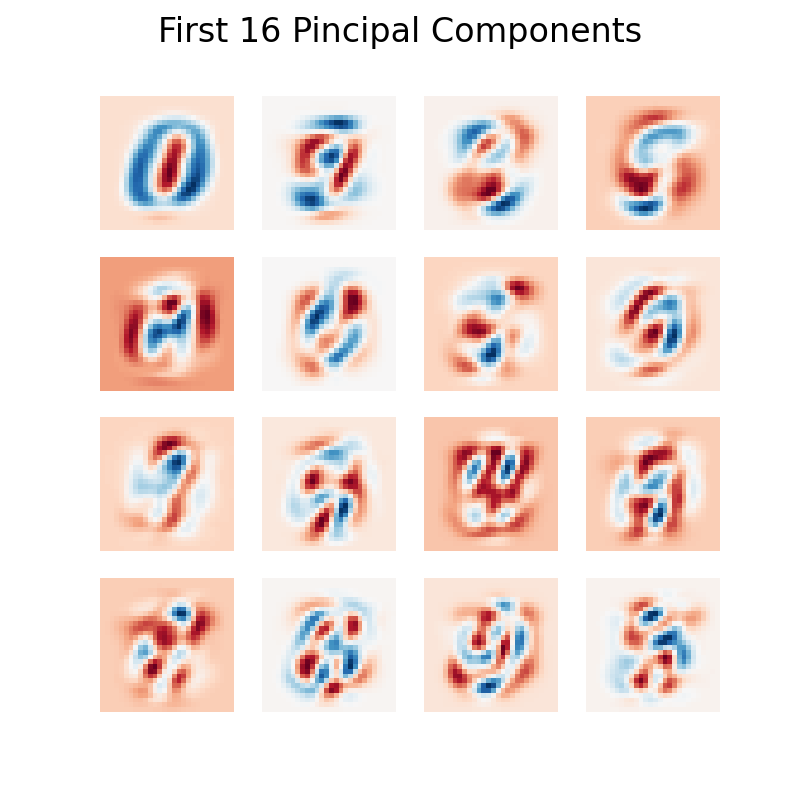
\includegraphics[width=.5\textwidth]{../visualizations/first_16_pincipal_components.png}
% 	\caption{ Here we have visualized the first 16 pc modes. These represent a basis for the 16 pc mode space where you can represent the image data as a linear combination of these modes.}\label{fig:f2}
%\end{figure}

\section{Summary and Conclusions}\label{sec:conclusions} 
\textbf{TODO: Update}

\section*{Acknowledgements}
\textbf{TODO: Update}
The author is thankful to Jaxon Tuggle, Hailey Sparks, Anja Vogt, Jade Glaister, and Nate Ward for offering regular feedback and counsel when interpreting results and clarifying the implications and merits of different classifiers.
We would also like to thank Professor Eli Shlizerman for carefully instructing us in class.

\bibliographystyle{abbrv}
\bibliography{references_hw4} % make sure this matches the .bib file for your corresponding document. You also have to maintain your references in the .bib file 

\end{document}
